\chapter{平面机构的结构分析(Structure Analysis of Planar Mechanisms)}
\intro{有机械者必有机事，有机事者必有机心。}
\rightline{————《庄子》}


\section{机构结构分析的目的和内容}
\textbf{目的}：研究机构组成的共同规律，建立一般分析方法。

\section{机构的组成}
\subsection{平面机构和空间机构}
\begin{itemize}
    \item \textbf{空间机构}：至少有两个构件在三维空间作相对运动的机构。
    \item \textbf{平面机构}：组成机构的各构件均在同一平面内或相互平行的平面内运动。
\end{itemize}

\subsection{运动副 (Kinematic Pair)}
两构件直接接触，又能容许一定的相对运动的连接。

\begin{itemize}
    \item \textbf{低副 (Low Pair)}：面接触,提供两个约束
    \begin{enumerate}
        \item 转动副 (revolute pair)：1 DOF
        \begin{figure}[htbp]
            \centering
            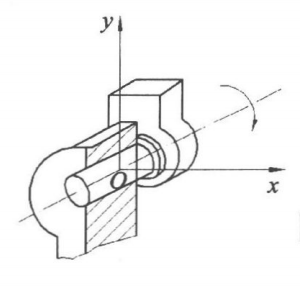
\includegraphics[width=0.2\textwidth]{figure/revolute_pair.png}
            \caption{转动副 (revolute pair)}
            \label{fig:revolute_pair}
        \end{figure}
        \item 移动副 (sliding pair)：1 DOF
        \begin{figure}[htbp]
            \centering
            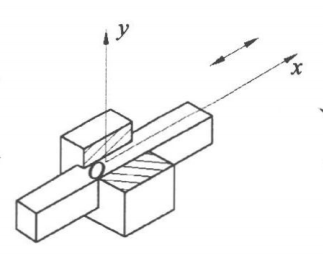
\includegraphics[width=0.2\textwidth]{figure/sliding_pair.png}
            \caption{移动副 (sliding pair)}
            \label{fig:sliding_pair}
        \end{figure}
    \end{enumerate}
    \item \textbf{高副 (High Pair)}：点/线接触,提供一个约束
    \begin{enumerate}
        \item 齿轮副 (gear pair)：2 DOF
        \begin{figure}[htbp]
            \centering
            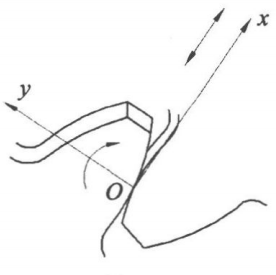
\includegraphics[width=0.2\textwidth]{figure/gear_pair.png}
            \caption{齿轮副 (gear pair)}
            \label{fig:gear_pair}
        \end{figure}
        \item 凸轮副 (cam pair)：2 DOF
        \begin{figure}[htbp]
            \centering
            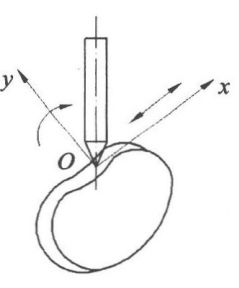
\includegraphics[width=0.2\textwidth]{figure/cam_pair.png}
            \caption{凸轮副 (cam pair)}
            \label{fig:cam_pair}
        \end{figure}
    \end{enumerate}
\end{itemize}

\subsubsection{自由度 (DOF)}
\begin{definition}
    构件含有独立运动的数目。
\end{definition}
\subsubsection{约束 (constraint)}
\begin{definition}
    对独立运动的限制。
\end{definition}

\subsection{运动链}
\begin{definition}
    两个以上的构件由运动副连接而成的系统。
\end{definition}

\begin{itemize}
    \item \textbf{闭链 (Closed chain)}
    \begin{definition}
        形成封闭回路的运动链。
\end{definition}
    \item \textbf{开链 (Open chain)}
    \begin{definition}
        未形成封闭回路的运动链。
\end{definition}
\end{itemize}
\[
\text{构件} + \text{运动副} = \text{运动链}
\]
\begin{remark}
    一个机构只有一个机架！
\end{remark}

\section{机构的运动简图 (Kinematic Diagram of Mechanism)}
\begin{remark}
    机构示意图和机构运动简图的区别：
    机构示意图只代表构件和运动副，不考虑运动副的相对位置。
    机构运动简图则考虑运动副的相对位置，更详细地表示机构的运动规律。
\end{remark}
\subsection{运动副表示方法}
\begin{enumerate}
    \item \textbf{转动副}  \textbf{轴线正确位置}：用圆圈表示转动中心，绘制两构件的相对位置。
    \begin{figure}[htbp]
        \centering
        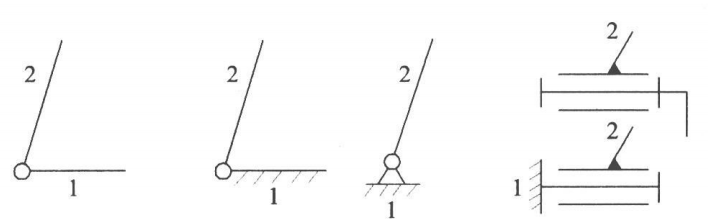
\includegraphics[width=0.5\textwidth]{figure/revolute_pair_draw.png}
        \caption{转动副运动简图}
    \end{figure}
    \item \textbf{移动副}  \textbf{相对移动方向}：用导路和滑块表示，突出移动方向。
    \begin{figure}[htbp]
        \centering
        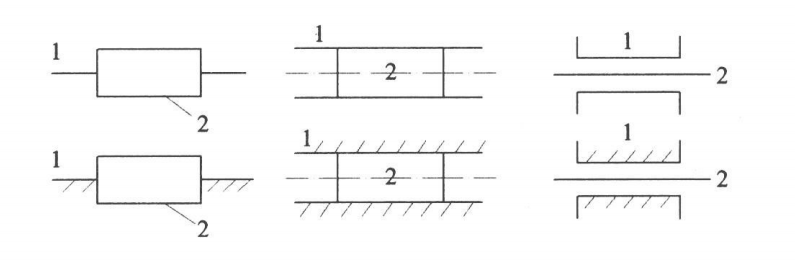
\includegraphics[width=0.5\textwidth]{figure/sliding_pair_draw.png}
        \caption{移动副运动简图}
    \end{figure}
    \item \textbf{齿轮副}  \textbf{相互接触部分}：用节圆或啮合线表示齿轮的啮合关系。
    \begin{figure}[htbp]
        \centering
        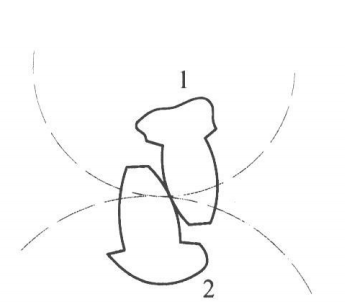
\includegraphics[width=0.5\textwidth]{figure/gear_pair_draw.png}
        \caption{齿轮副运动简图}
    \end{figure}
    \item \textbf{凸轮副}  \textbf{相互接触的曲线轮廓}：绘制凸轮轮廓与从动件的接触形态。
    \begin{figure}[htbp]
        \centering
        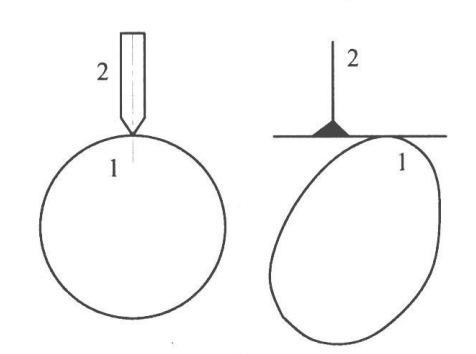
\includegraphics[width=0.5\textwidth]{figure/cam_pair_draw.png}
        \caption{凸轮副运动简图}
    \end{figure}
\end{enumerate}

\subsection{构件的表示方式}
不考虑与运动无关的因素（如无关外形等），核心是表达构件间的连接关系。
原则：会画就会看，会看就会画。

\subsection{画机构运动简图的一般步骤}
\begin{figure}[htbp]
    \centering
    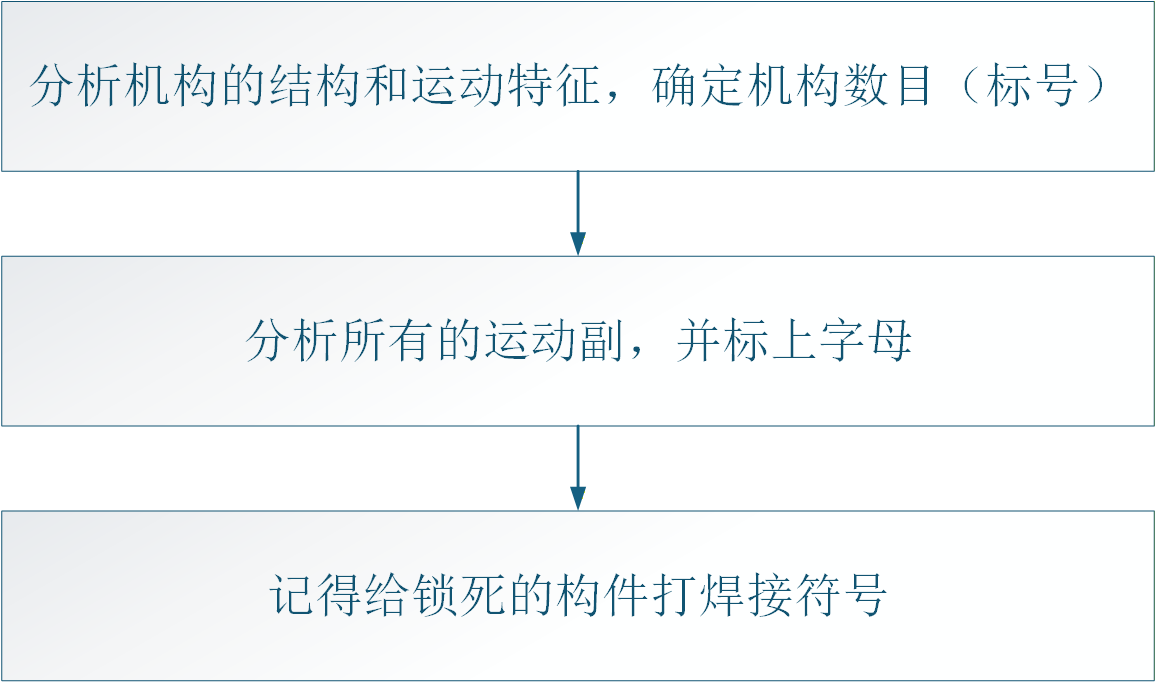
\includegraphics[width=0.5\textwidth]{figure/机构简图绘制流程.png}
    \caption{机构运动简图的一般步骤}
\end{figure}
\section{机构的自由度}
平面机构自由度计算公式：
\[
DOF = 3n - 2P_L - P_H
\]
其中：
\begin{itemize}
    \item \(n\)：活动构件个数
    \item \(P_L\)：低副个数
    \item \(P_H\)：高副个数
\end{itemize}

\subsubsection{机构具有确定运动的条件}：
\[
\begin{cases}
DOF > 0 \\
\text{原动件数} = \text{机构的自由度}
\end{cases}
\]

\subsection{复合铰链(Compound Hinge)}
\(k\) 个构件组成的复合铰链，应将 \(k-1\) 个转动副计入计算。

\subsection{局部自由度(Passive DOF)}
存在与否不影响整个机构的运动规律，计算自由度之前先去除局部自由度（常为滚轮结构）。处理方法：焊死即可。

\subsection{虚约束 (Redundant Constraints)}
某些约束对机构的限制作用或自由度的影响是重复的，即不起独立限制作用的约束。计算时需摘掉构件和约束（有限定几何条件，一般情况）。

\subsection{常见情况}
\begin{enumerate}
    \item 不同构件上两点间距、距离保持恒定。
    \item 两构件构成多个移动副且导路互相平行。
    \item 两构件构成多个转动副且轴线相互重合。
    \item 在输入件与输出件之间用多组完全相同的运动链来传递运动，只有一组起独立传递运动的作用，其余引入虚约束。
\end{enumerate}

\section{自由度计算的步骤}
\begin{figure}[htbp]
    \centering
    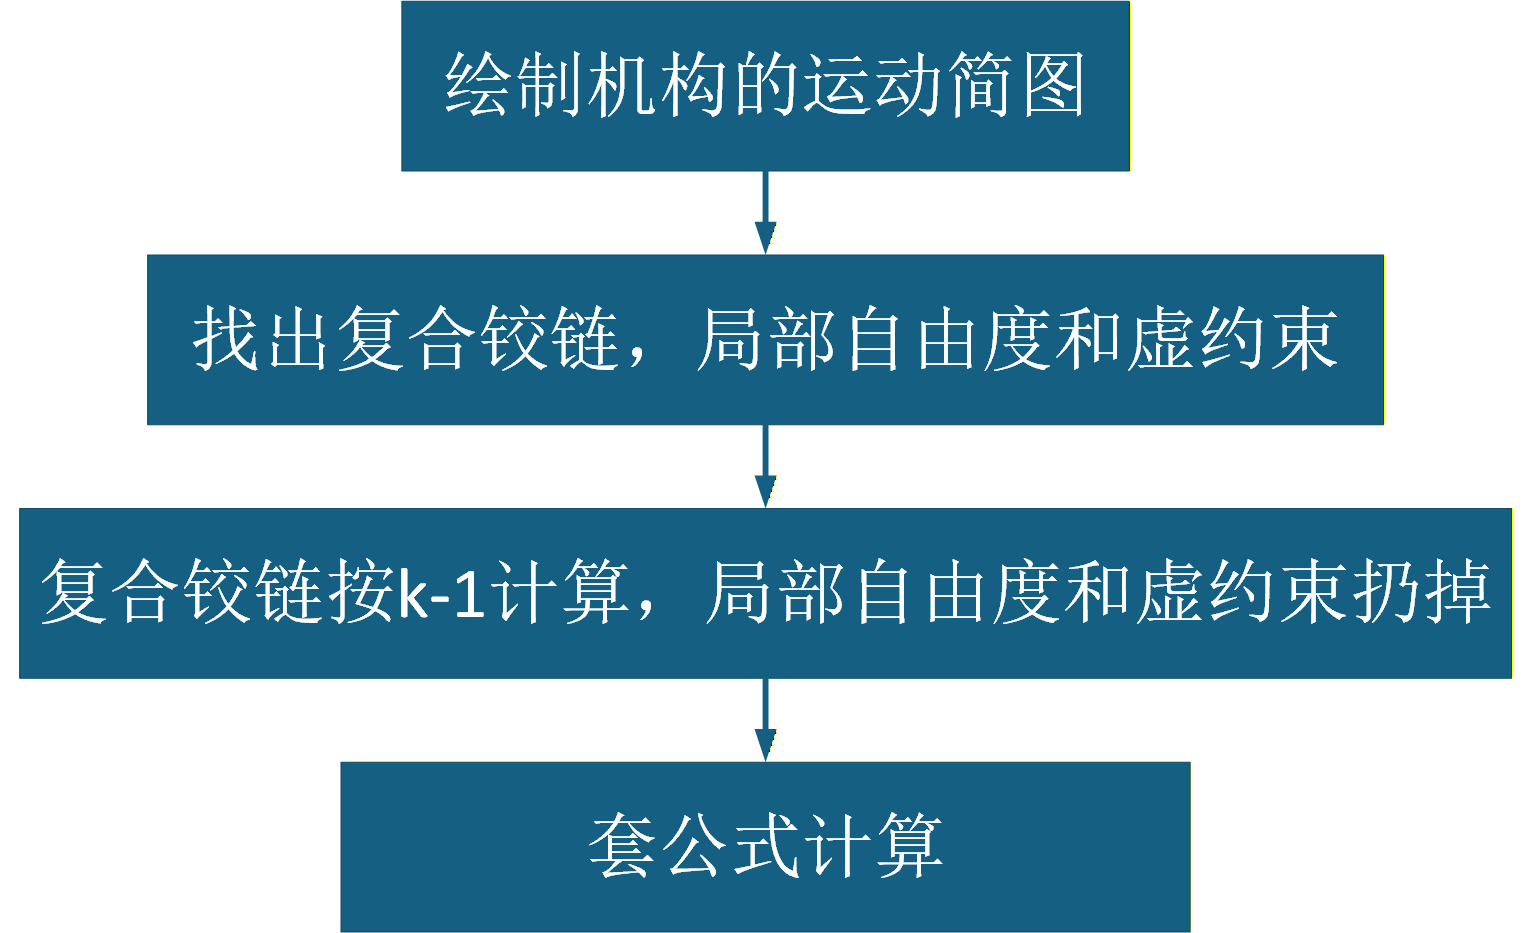
\includegraphics[width=0.8\textwidth]{figure/自由度计算步骤.png}
    \caption{自由度计算的步骤}
\end{figure}
